\reportheading{3. Diffuser selection and peak throw (Task 1)}
\subhead{3.1 Neck selection on the adopted ceiling grid}
The Krueger 1400/51400 four-cone outlet distributes supply air along both ceiling axes. For the 600 mm square panel without a damper, we compared the metric catalogue tables [2] at the same outlet positions and flows. For each operating flow, we interpolated the third horizontal isothermal throw between adjacent catalogue rows and divided the resulting throw by the directional length. Peak outlet flows span 134.22–202.19 L/s; minimum flows span 53.69–80.88 L/s.

\tabletitle{Table 3. Neck comparison using the adopted flows and geometry.}
\begin{reporttable}{L{.15}L{.22}L{.23}L{.40}}
\rowcolor{tablegrey} Neck & Lowest T/L & Highest T/L & Selection consequence \\\hline
6 inch & 1.2078 & 3.4476 & Peak flow approaches catalogue maximum of 204 L/s. \\
8 inch & 1.1608 & 3.4 (rounded) & Retains minimum-flow reach with a smaller peak exceedance. \\
10 inch & 0.9724 & 3.4325 & Falls below 1.0 at minimum flow. \\
\end{reporttable}
The 12-, 14- and 15-inch tables begin at 74, 101 and 116 L/s respectively, above the lowest required flow. At the highest outlet flow of 202.19 L/s, the 6-inch neck is already close to its last catalogue row (204 L/s). Increasing the neck to 10 inches creates a different difficulty: its lowest throw ratio falls to 0.9724 at turndown. The selected 8-inch neck keeps the low-flow ratio above 1.0, although the two facing wing outlets still slightly exceed the upper limit at peak flow.

\subhead{3.2 Peak-load check}
For SD-77 east and SD-78 west, the catalogue throw lies between 5.1 m at 198 L/s and 5.5 m at 231 L/s: $T_{0.25}=5.1+(202.189-198)(0.4/33)=5.151$ m. Dividing by 1.500 m gives a peak ratio of 3.4 to one decimal place. The unrounded value in Appendix A is slightly above the selection limit of 3.4.
{\centering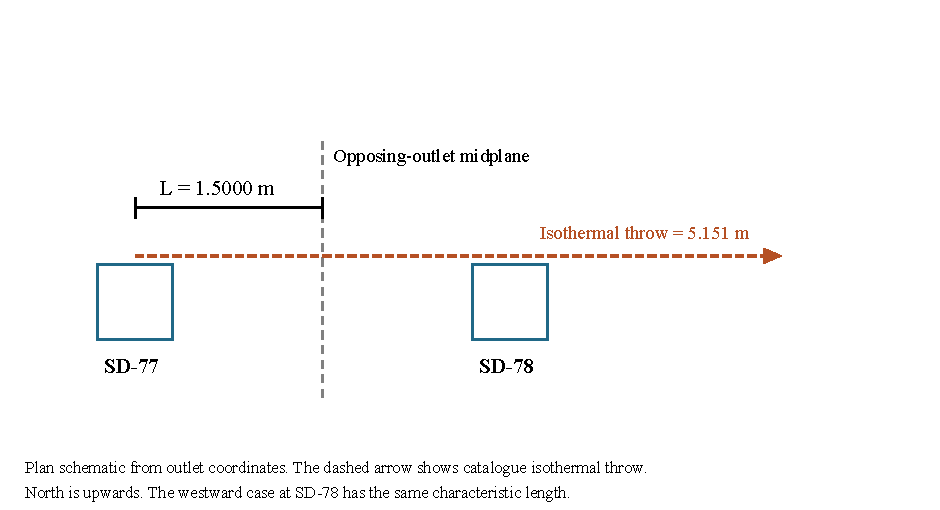
\includegraphics[width=.71\linewidth]{figures/critical-case.pdf}\par}
\reportfigure{}{Figure 1. Peak throw and opposing-outlet midplane at SD-77.}

On this pair of tiles, the upper ratio corresponds to a catalogue throw of $3.4\times1.500=5.100$ m. The interpolated throw extends about 51 mm beyond that value. This is a catalogue margin at the midplane.
